\part*{Lektion 8: NumPy und Matplotlib}
\section{NumPy}
\begin{itemize}
	\item Python-Bibliothek
	\item[\-] \texttt{import numpy as np}
	\item Einfache Handhabung mit Vektoren und Matrizen
	\begin{itemize}
		\item mehrdimensionale Arrays
	\end{itemize}
	\item Funktionen für numerische Berechnungen
	\begin{itemize}
		\item Grundlegende Operationen
		\item Mathematische Funktionen (sin, cos, sqrt, exp, ...)
		\item Lineare Algebra
		\item ...
	\end{itemize}
	\item Effiziente und schnelle Ausführung
	\begin{itemize}
		\item kompilierte Funktionen und Algorithmen
		\item Array-basierte Operationen $\rightarrow$ keine \texttt{for}-Schleifen
	\end{itemize}
	\item Ähnlichkeit zu MATLAB\textsuperscript{\textregistered}
	\item[\-] \url{https://docs.scipy.org/doc/numpy/user/ numpy-for-matlab-users.htm}
\end{itemize}

\subsection{ndarray erzeugen}
\begin{itemize}
	\item N-dimensionales Array (\url{https://docs.scipy.org/doc/numpy/reference/generated/numpy.ndarray.html})
	\item ndarray erzeugen\\
	\lstinputlisting{listings/v8_numpy1.py}
	\item Weitere Funktionen, um Arrays zu erzeugen\\
	\begin{tabular}{|l|l|}
		\hline 
		\textbf{Funktion} &\textbf{Resultat}\\ 
		\hline 
		\texttt{np.arange(3)} &\texttt{array([0, 1, 2])}\\ 
		\texttt{np.ones((2,2))} &\texttt{array([[1., 1.], [1., 1.]])}\\ 
		\texttt{np.ones\_like(arr1)} &\texttt{array([1, 1, 1])}\\ 
		\texttt{np.zeros((2,2))} &\texttt{array([[0., 0.], [0., 0.]])}\\ 
		\texttt{np.zeros\_like(arr1)} &\texttt{array([0, 0, 0])}\\ 
		\texttt{np.full((2,2), 7.0)} &\texttt{array([[7., 7.], [7., 7.]])}\\ 
		\texttt{np.full\_like(arr1, 7)} &\texttt{array([7, 7, 7])}\\ 
		\texttt{np.eye(2)} &\texttt{array([[1., 0.], [0., 1.]])}\\ 
		\texttt{np.identity(2)} &\texttt{array([[1., 0.], [0., 1.]])}\\ 
		\texttt{np.linspace(0, 1, 5)} &\texttt{array([0., 0.25, 0.5, 0.75, 1.])}\\ 
		\texttt{np.logspace(0, 1, 4)} &\texttt{array([1., 2.1544, 4.6416, 10.])}\\ 
		\texttt{np.random.randn(3)} &\texttt{array([0.7576, 0.0135, -0.8934])}\\ 
		\hline 
	\end{tabular} 
\end{itemize}

\subsubsection{ndarray-Datentypen}
\begin{itemize}
	\item Datentyp wird automatisch ermittelt,\\
	z.B. \texttt{np.int64} oder \texttt{np.float64}
	\item Datentyp erzwingen\\
	\texttt{np.array([1, 2, 3], dtype=np.complex)}
	\item Mögliche Datentypen\\
	\begin{tabular}{|l|l|}
		\hline 
		\texttt{np.int8, np.uint8} &8-Bit Ganzzahlen\\ 
		\texttt{np.int16, np.uint16} &16-Bit Ganzzahlen\\ 
		\texttt{np.int32, np.uint32} &32-Bit Ganzzahlen\\ 
		\texttt{np.int64, np.uint64} &64-Bit Ganzzahlen\\ 
		\texttt{np.float16} &Float mit halber Genauigkeit\\ 
		\texttt{np.float32} &Float mit einfacher Genauigkeit\\ 
		\texttt{np.float64} &Float mit doppelter Genauigkeit\\ 
		\texttt{np.float128} &Float mit vierfacher Genauigkeit\\  
		\texttt{np.complex64/128/256} &Komplexe Zahl\\ 
		\texttt{np.bool} &Boolescher Wert, True/False\\ 
		\hline 
	\end{tabular} 
\end{itemize}

\subsection{Arithmetische Operationen}
\begin{itemize}
	\item Arithmetische Operationen werden elementweise ausgeführt\\
	\lstinputlisting{listings/v8_numpy2.py}
	\begin{tabular}{|l|l|}
		\hline
		\textbf{Operation} &\textbf{Resultat}\\
		\hline
		\texttt{arr + arr} &\texttt{array([2., 4., 6.])}\\
		\texttt{arr + 1} &\texttt{array([2., 3., 4.])}\\
		\texttt{arr - arr} &\texttt{array([0., 0., 0.])}\\
		\texttt{arr - 1} &\texttt{array([0., 1., 2.])}\\
		\texttt{arr*arr} &\texttt{array([1., 4., 9.])}\\
		\texttt{arr*2} &\texttt{array([2., 4., 6.])}\\
		\texttt{arr/arr} &\texttt{array([1., 1., 1.])}\\
		\texttt{arr/2} &\texttt{array([0.5, 1., 1.5])}\\
		\texttt{arr**2} &\texttt{array([1., 4., 9.])}\\
		\texttt{arr > 2} &\texttt{array([False, False, True], dtype=bool)}\\
		\hline
	\end{tabular}
\end{itemize}

\vfill\null
\pagebreak
\subsection{Indexierung}
\begin{multicols}{2}
	\begin{itemize}
		\item Indexierung von 2D-Arrays\\
		\lstinputlisting{listings/v8_numpy3.py}
		\item Beispiele:\\
		\lstinputlisting{listings/v8_numpy4.py}
	\end{itemize}
	\columnbreak
	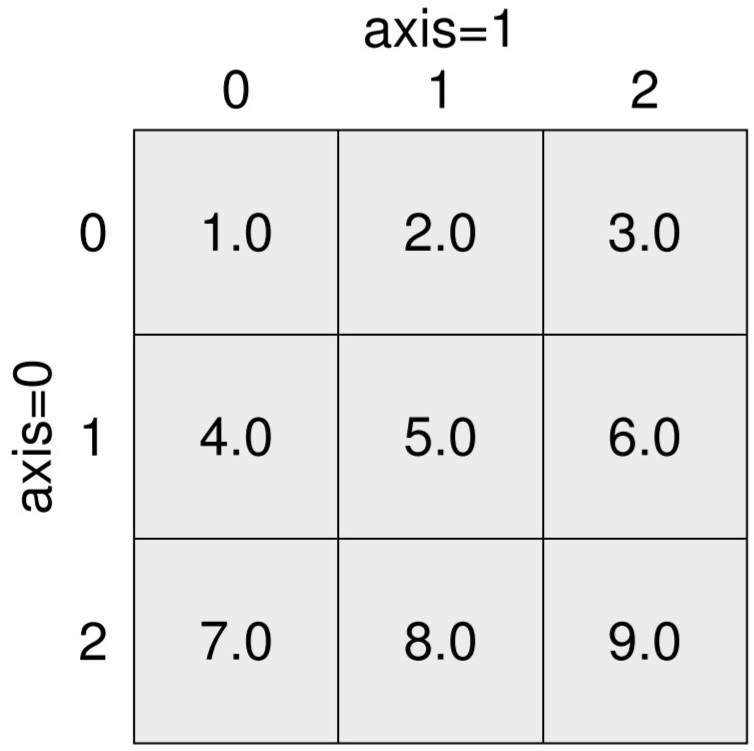
\includegraphics[width=0.7\linewidth]{images/v8_numpy1}
\end{multicols}

\subsubsection{Slicing}
\begin{tabular}{|l|l|l|l|}
	\hline
	\texttt{arr} &Ausdruck &Shape &Resultat\\
	\hline
	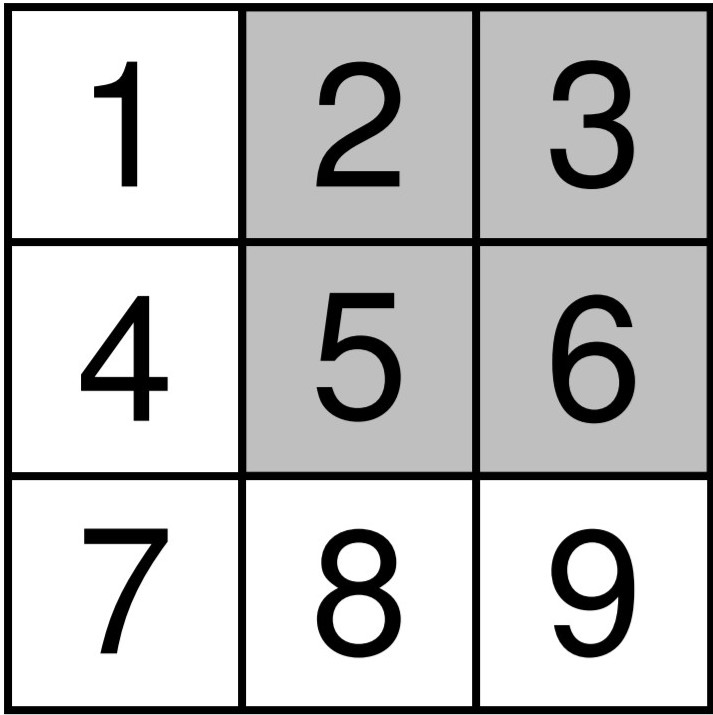
\includegraphics[width=0.1\linewidth]{images/v8_numpy2} &\texttt{arr[:2, 1:]} &(2,2) &\texttt{array([[2, 3], [5, 6]])}\\
	\hline
	\multirow{3}{0.1\linewidth}{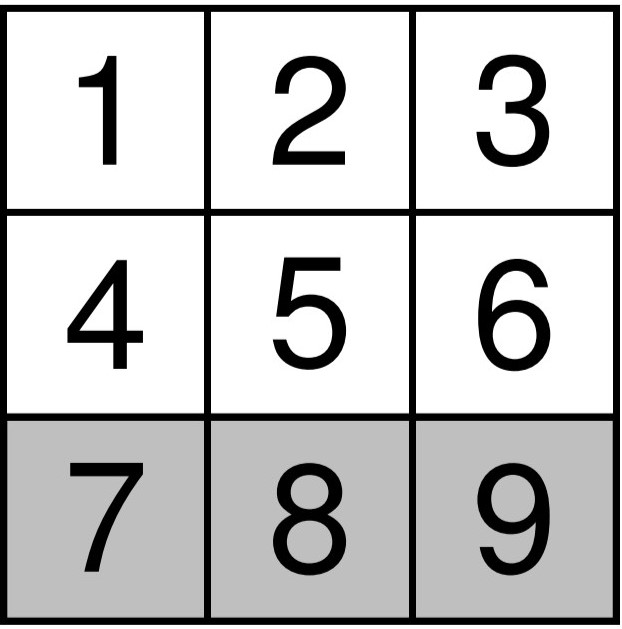
\includegraphics[width=\linewidth]{images/v8_numpy3}} &\texttt{arr[2]} &(3, ) &\texttt{array([7, 8, 9])}\\
	&\texttt{arr[2, :]} &(3, ) &\texttt{array([7, 8, 9])}\\
	&\texttt{arr[2:, :]} &(1, 3) &\texttt{array([[7, 8, 9]])}\\
	\hline
	\multirow{3}{0.1\linewidth}{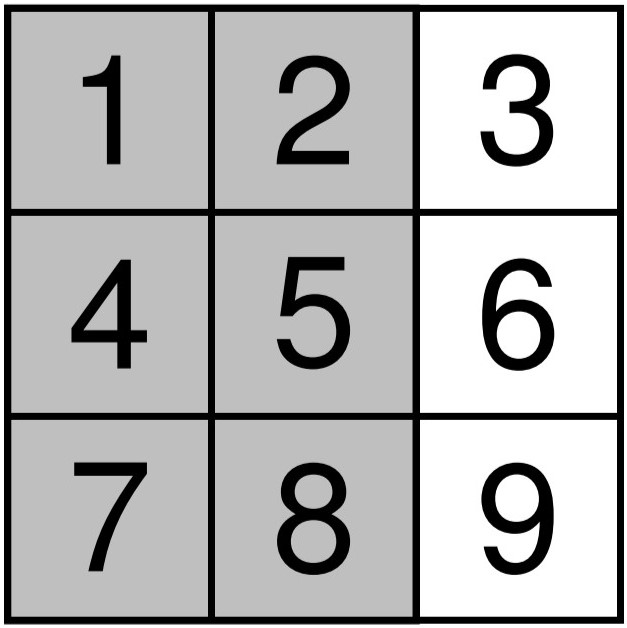
\includegraphics[width=\linewidth]{images/v8_numpy4}} &\texttt{arr[:, :2]} &(3, 2) &\texttt{array([[1, 2],}\\
	& & &\texttt{[4, 5],}\\
	& & &\texttt{[7, 8]])}\\
	\hline
	\multirow{3}{0.1\linewidth}{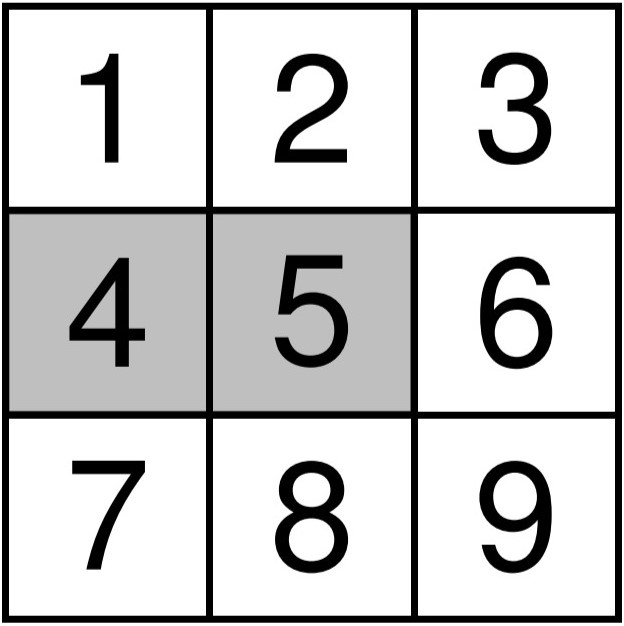
\includegraphics[width=\linewidth]{images/v8_numpy5}} &\texttt{arr[1, :2]} &(2, ) &\texttt{array([4, 5])}\\
	&\texttt{arr[1:2, :2]} &(1, 2) &\texttt{array([[4, 5]])}\\
	& & &\\
	\hline
\end{tabular}\\
$\rightarrow$ \texttt{ndim} bleibt erhalten, falls bei jeder \texttt{axis} ein $"$:$"$ steht.
\begin{itemize}
	\item Ein Slice ist immer eine Referenz, keine Kopie!
	\lstinputlisting{listings/v8_numpy5.py}
	\item Kopien werden mit \texttt{.copy()} erzeugt:
	\lstinputlisting{listings/v8_numpy6.py}
	\item Zuweisung eines Skalars zu einem Slice wird ausgebreitet:
	\lstinputlisting{listings/v8_numpy7.py}
	\item Bei fehlender Dimension wird das Array automatisch erweitert:
	\lstinputlisting{listings/v8_numpy8.py}
\end{itemize}
$\rightarrow$ Bedingung: letzte Dimension ist gleich oder nur 1 lang.

\subsection{Mathematische Funktionen}
\begin{itemize}
	\item NumPy beinhaltet viele mathematische Funktionen:\\
	\url{https://docs.scipy.org/doc/numpy/reference/routines.math.html}
	\begin{itemize}
		\item \texttt{np.sin()}
		\item \texttt{np.cos()}
		\item \texttt{np.exp()}
		\item \texttt{np.cumsum()}
		\item ...
	\end{itemize}
	\item Diese Funktionen operieren über das gesamte Array
	\lstinputlisting{listings/v8_numpy9.py}
\end{itemize}

\subsubsection{Lineare Algebra}
\begin{itemize}
	\item Liste der Funktionen:\\
	\url{https://docs.scipy.org/doc/numpy/reference/routines.linalg.html}
	\item Matrix definieren
	\lstinputlisting{listings/v8_numpy14.py}
	\item Vektor definieren
	\lstinputlisting{listings/v8_numpy15.py}
	\item Matrix \textbf{M} mit Vektor \textbf{v} multiplizieren
	\lstinputlisting{listings/v8_numpy10.py}
	\item Matrix transponieren \textbf{M$^T$}
	\lstinputlisting{listings/v8_numpy11.py}
	\item Matrix invertieren \textbf{M$^{-1}$}
	\lstinputlisting{listings/v8_numpy12.py}
	\item Shape eines Vektors ändern
	\lstinputlisting{listings/v8_numpy16.py}
\end{itemize}

\subsubsection{Matplotlib}
\begin{itemize}
	\item Python-Bibliothek\\
	\texttt{import matplotlib.pyplot as plt}
	\item Erstellen von publizierbaren Diagrammen und Darstellungen
	\item 100\% kompatibel zu NumPy-Arrays
	\item MATLAB\textsuperscript{\textregistered}-ähnliche Funktionen:\\
	\url{https://matplotlib.org/api/_as_gen/matplotlib.pyplot.html}
	\item Kann auch objekt-orientiert verwendet werden, z.B. in GUIs
	\item Grosse Beispiel-Sammlung:\\
	\url{https://matplotlib.org/gallery/index.html}
	\item Einfaches Beispiel:
\end{itemize}
\begin{multicols}{2}
	\lstinputlisting{listings/v8_numpy13.py}
	\vfill\null
	\columnbreak
	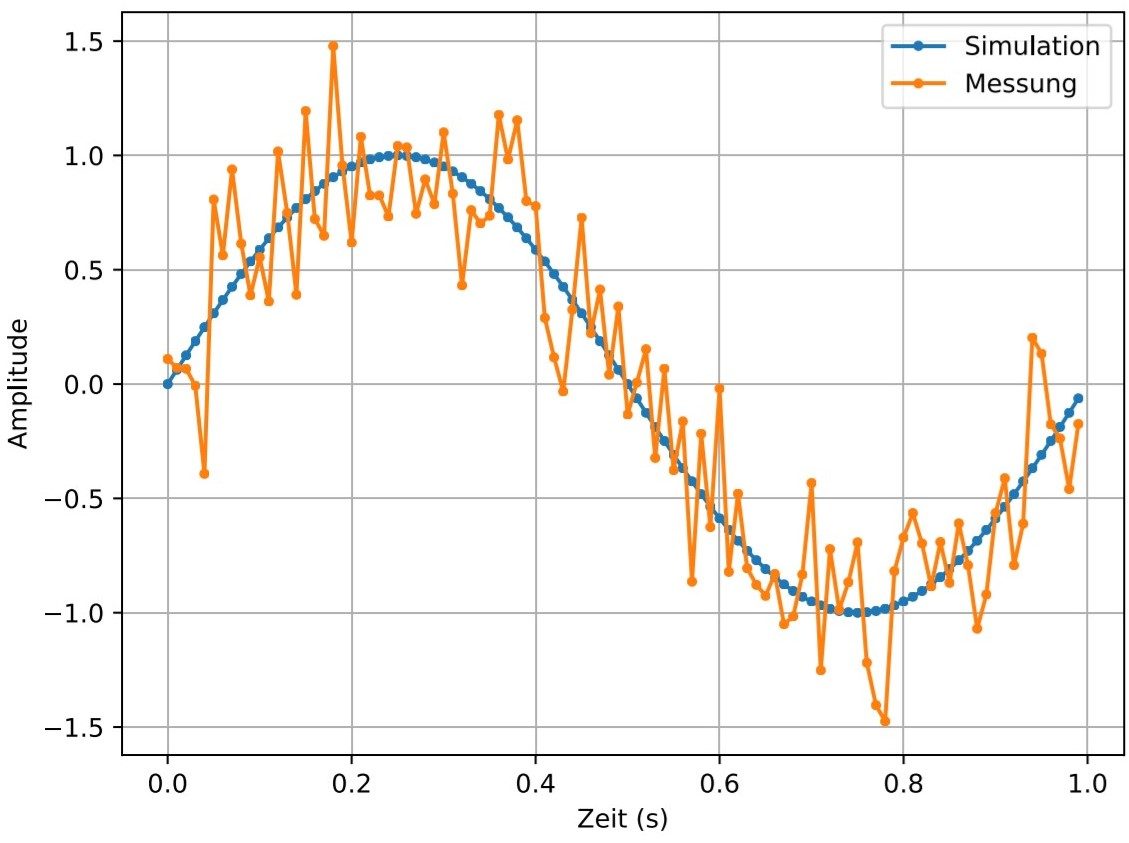
\includegraphics[width=\linewidth]{images/v8_numpy6}
\end{multicols}